\chapter{Architecture and Design}
\label{chapter:architecture}

Before we reach the point of discussing a new future-proof, modern architecture and design of Tribler, the evolution of the Tribler architecture  throughout the last 10 years will be elaborated. Understanding the past decisions regarding architecture and design, will help us to shed light on the question why Tribler has accumulated such an amount of technical debt.\\\\
According to OpenHub, Tribler has a total of 111 unique contributors so far\cite{openhubtribler}. This list is most likely not complete since some work of missing contributors might have been finished by another member of the Tribler team. Searching for \emph{Tribler} in the TU Delft repository, results in a total of 66 hits of which 35 results are contributions in the form of a MSc or BSc thesis.\\\\
The remaining of this chapter will present a historical description of the evolution of Tribler. The purpose is to present a historical evolution of the code base so we can better understand the design decisions made in the past and how they might have led to the present state of the system.

\section{Tribler: A social-based peer-to-peer system}
In April 2005, Tribler started out as fork from \emph{Another BitTorrent Client} (ABC), an improved BitTorrent client. ABC is based on \emph{BitTornado} which extended from the \emph{BitTorrent} core system, written by Bram Cohen. In the current code base of Tribler, various references to ABC can be found, mostly notable in the naming of files, variables and classes.\\\\
In 2007, the first major research paper was published, describing Tribler as a social-based peer-to-peer system\cite{pouwelse2008tribler}. The key idea is that social connections between peers in a decentralized network can be exploited to increase usability and performance of the network. This is based on the idea that peers belonging to a social group are not likely to steal (free-ride) bandwidth from each other. The system architecture of the system is visible in Figure \ref{fig:tribler-architecture-2008}. In the remainder of this Section, the most important components of the architecture as described in \cite{pouwelse2008tribler} will be explained in more detail.

\begin{figure}[t]
	\centering
	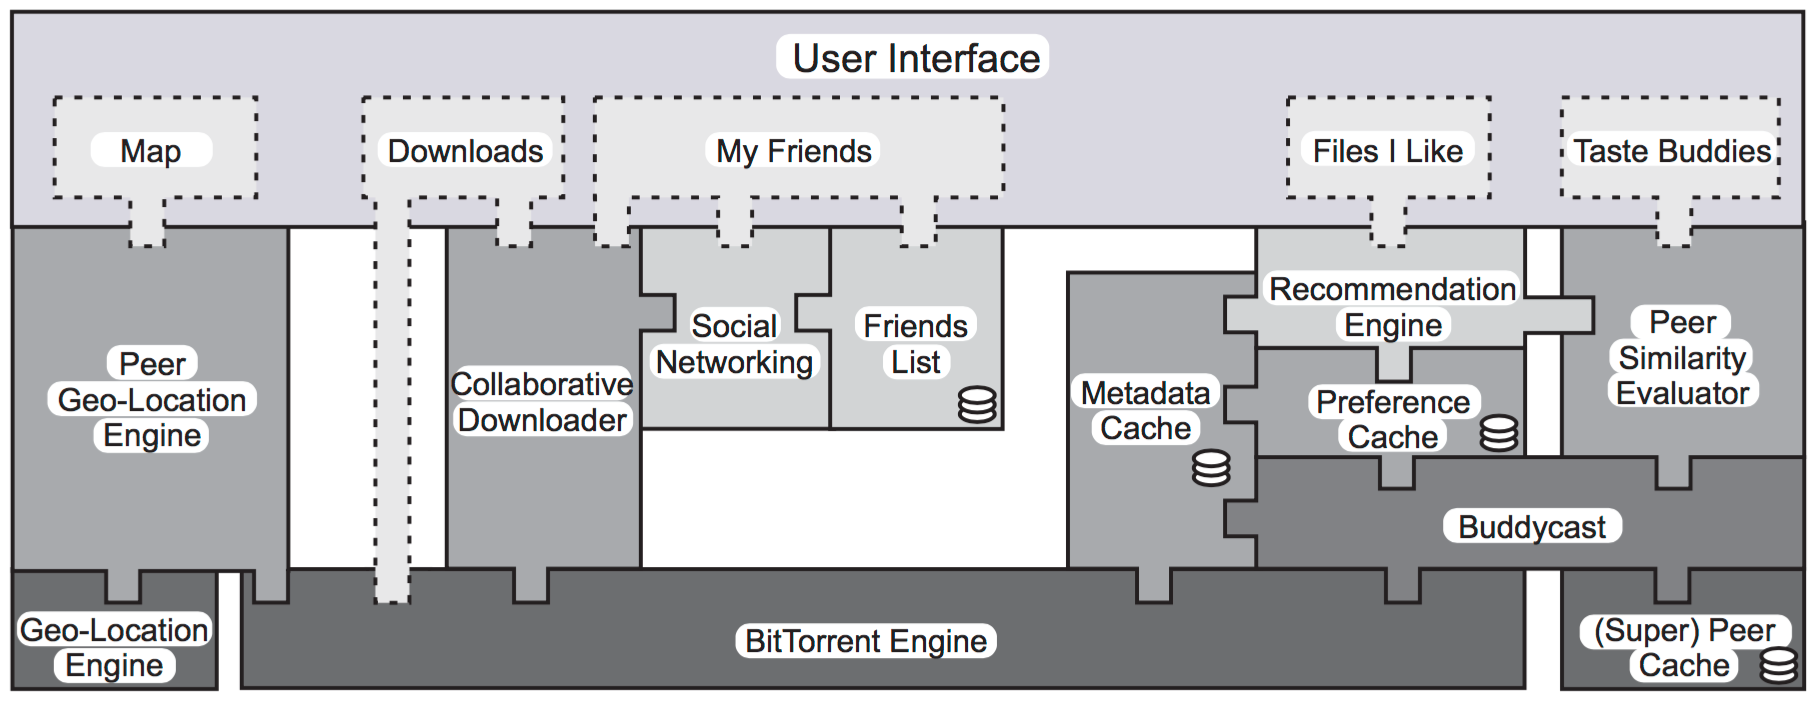
\includegraphics[width=0.9\columnwidth]{images/tribler_architecture_2007}
	\caption{The system architecture as described in \cite{pouwelse2008tribler}.}
	\label{fig:tribler-architecture-2008}
\end{figure}

\subsection{Collaborative Downloads}
The BitTorrent engine allows the mechanism to download and seed torrent files using a BitTorrent-compatible protocol. In addition, the module allows usage of the \emph{collaborative downloader} module which significantly increases download speed by exploiting idle upload capacity of online friends.\\\\
The protocol to facilitate collaborative downloads is called \emph{2Fast} and the idea is that a user invokes the help of friends to increase download speed of his files. The protocol uses social groups where members who trust each other collaborate to improve their download performance. Peers that are participating in a social group are either \emph{collectors} or \emph{helpers}. A collector is a peer that is interested in obtaining a complete copy of a particular file. A helper is a peer that is recruited by a collector to help downloading that file.

\subsection{Peer Geo-Location Engine}
The \emph{Peer Geo-Location Engine} is an engine built on top of a module that enables geographical lookup of IP addresses (\emph{http://hostip.info}). When a peer downloads a file, peers in the download swarm are displayed on a map in the user interface.

\subsection{Content Discovery and Recommendation}
The \emph{BuddyCast} algorithm is designed to make recommendations and to enable peer and content discovery. BuddyCast is an epidemic protocol which works as follows: each peer in the network maintains a number of taste buddies with their preference lists and a numer of random peers without any information about their preferences. Periodically, an \emph{exploration} or \emph{exploitation} step is performed. When an exploration is executed, the peer connects to one of its taste buddies. The peer connects to a random peer if an exploitation step is performed. When the connection is successful, a \emph{BuddyCast} message is exchanged.\\\\
A Buddycast message contains the identities of a number of taste buddies along with their top-10 preference lists, a number of random (and fresh, see below) peers, and the top-50 preferences of the sending peer. The age of each peer is included in the message to help others know the freshness of peers. After the BuddyCast messages are exchanged, the received information is stored in the local database of each peer. To limit redundant messages, each peer maintains a list of recently contacted peers.

\section{Tribler in 2007 and onwards}
The next version of Tribler, version 4.0, got released in 2007\cite{tribler4tf}. Many features from the 3.x release cycles are taken over and some new functionality have been added. Using an embedded video player, users can play videos (while being downloaded) directly from within the user interface. This video player is powered by the VLC library and bindings for the user interface library, \emph{wxPython}. Tribler 4.0 allows users to remotely search for content inside the Tribler network but also content on YouTube and Liveleak. The search results are displayed in a YouTube-like thumbnail grid. The interface of Tribler 4.0 is displayed in Figure \ref{fig:tribler4}.

\begin{figure}[t]
	\centering
	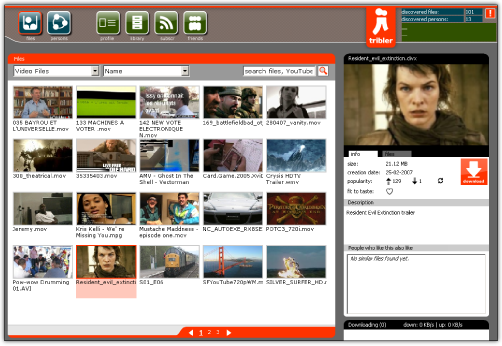
\includegraphics[width=0.8\columnwidth]{images/tribler4}
	\caption{The user interface of Tribler 4.0.}
	\label{fig:tribler4}
\end{figure}

\subsection{Tribler 5.x}
The development of Tribler continued with the release of Tribler 5.0 in 2009\cite{historyoftribler}. The interface got a complete overhaul, introducing a more dark theme, which was replaced by a white theme a short while after the release. In the 5.x series, several improvements to Tribler itself and the user interface has been made. The focus of Tribler 5.0 has been on remote search and downloads. The thumbnails have been dropped and the search results are displayed in a paginated list instead.\\\\
Tribler 5.1 contained some major improvements to the user interface, thanks to the feedback of the community. A new major addition have been added to Tribler 5.2: the concepts of channels, similar to YouTube, has been introduced. One goal of channels was to prevent spam inside the network by favouring content in more popular channels. The popularity indicator associated with each torrent got removed but has been placed back later. In Tribler 5.3, all custom widgets got replaced by native buttons, creating a more native feel on each platform. A tag cloud has been added to the home page of Tribler to help users determine which content they possibly want to look for. Moreover, the paginated list was replaced by a single, scrollable list of items. Tribler 5.4 introduced a magic search feature where similar search results are collapsed using text similarity functions and digit extraction. This leads to a much cleaner and comprehensive results list when searching.\\\\
The final release in the 5.x series, Tribler 5.9, bought some major additions. The complete BuddyCast core has been rewritten, moving away from a TCP overlay to an implementation based on UDP, bringing huge benefits to the compatibility with NAT-firewalls. Also, \emph{libswift} has been introduced as the new download engine, providing download capabilities over UDP, removing the TCP layer from libtorrent.

\section{Tribler 6.x}
Shortly after the release of Tribler 5.9, Tribler 6.0 is released where a complete new user interface has been implemented. This version contained also some minor bug fixes that increased performance and usability. After the release of 6.0.1, several smaller releases (6.1, 6.2 and 6.3) were released. The focus shifted toward anonymous downloads and end-to-end encryption. These features were part of the Tribler 6.4 release, providing an experimental anonymous download mechanism and hidden seeding services. Moreover, the \emph{libswift} dependency got dropped since it was not stable enough. This release also introduced the Trivial File Transfer Protocol (TFTP), used to transfer torrent files between peers in Tribler. The next release, Tribler 6.4.1, contained some major security fixes after an external code review.

\section{The roadmap of Tribler}
In the previous Section, the evolution of Tribler has been evolved, up to the current architecture. We now turn our attention to the future of Tribler and propose a new architecture that will enable Tribler for another 10 year of research. The proposed architecture is visible in Figure \ref{fig:tribler7}. This architecture follows a layered approach with a clear distinction between the visible layers. This Section will discuss the proposed design and highlight decisions that have been made during the development process.

\begin{figure}[h!]
	\centering
	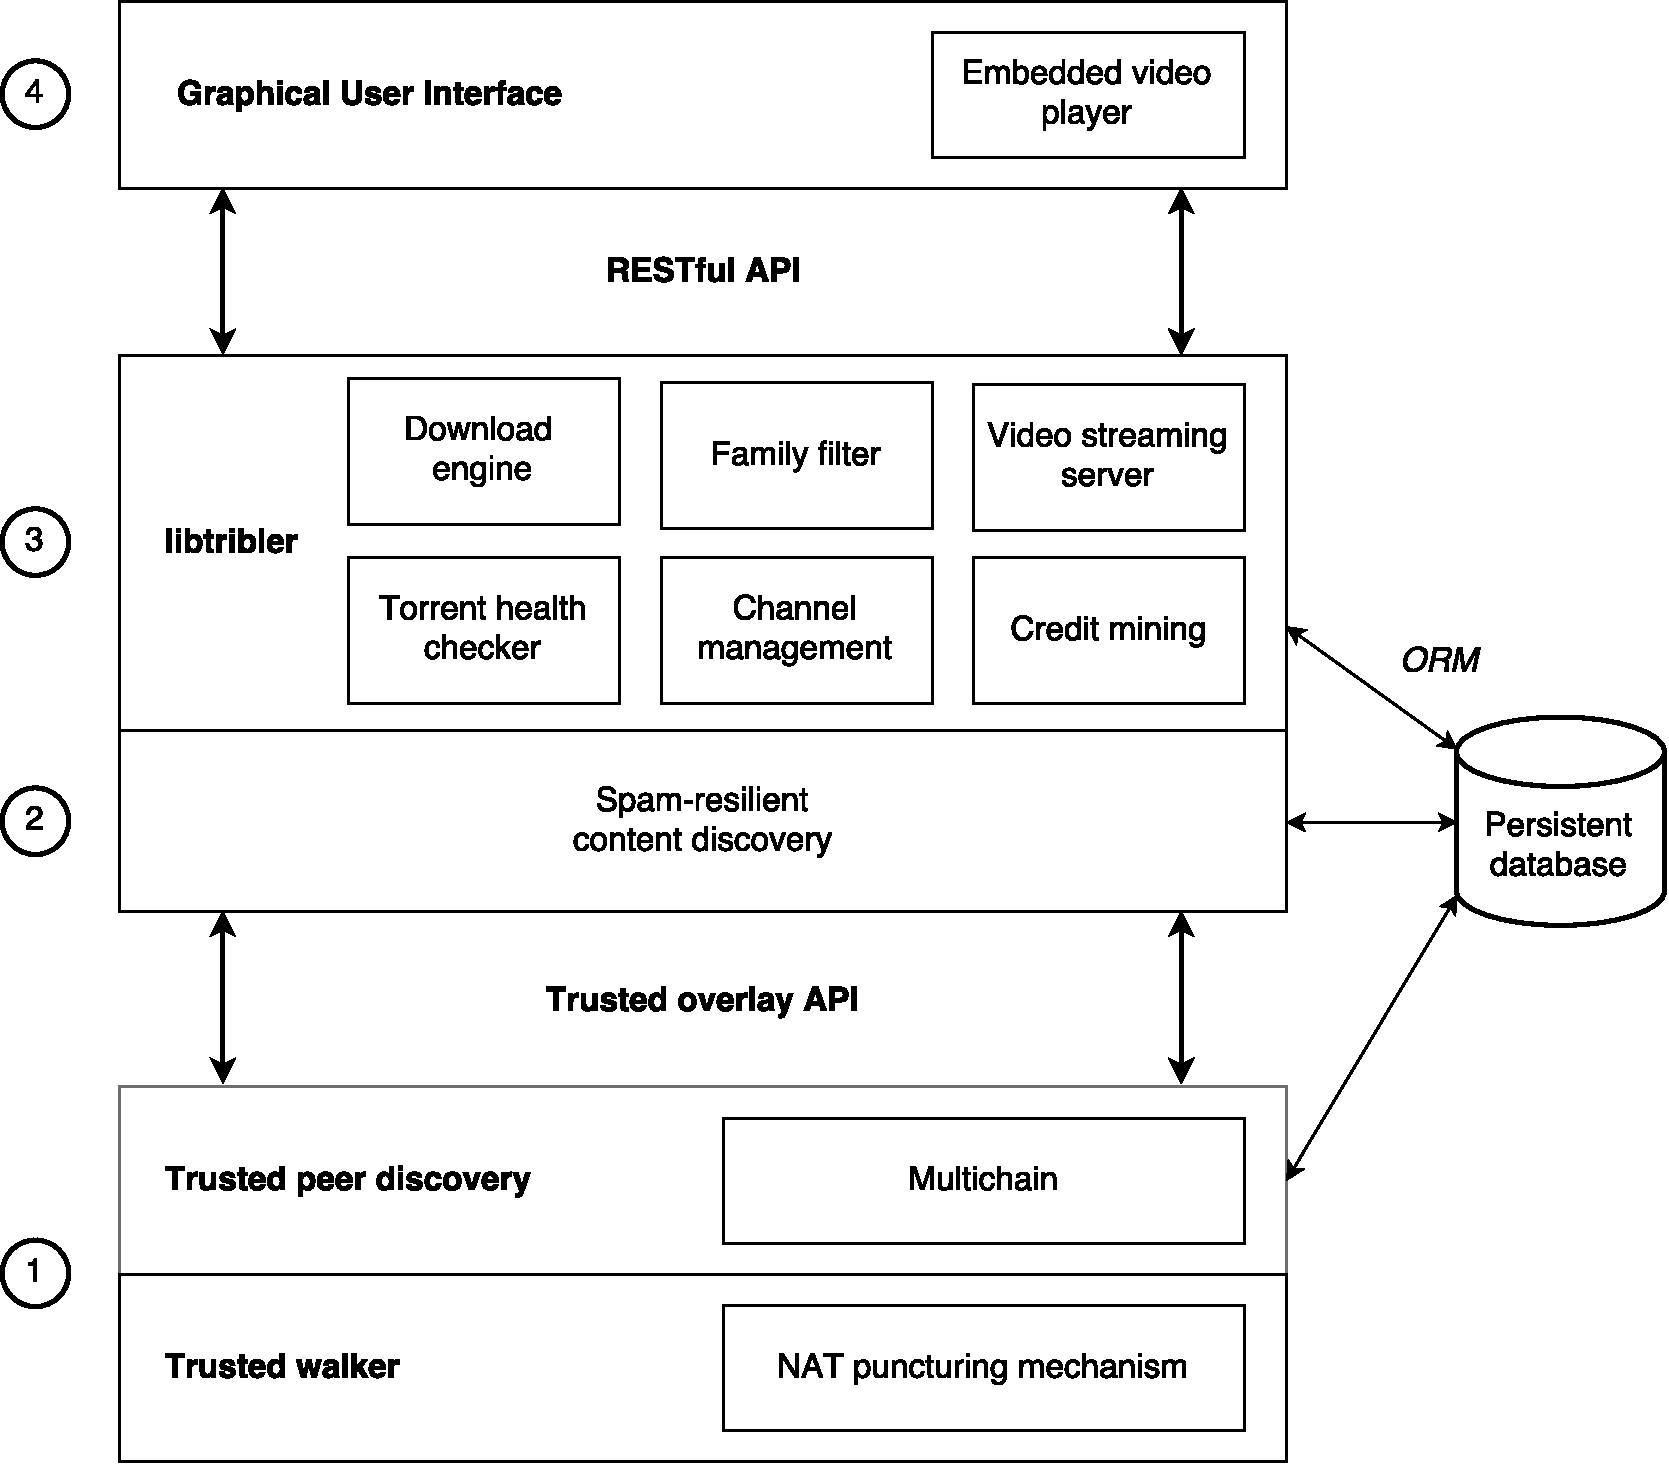
\includegraphics[width=0.7\columnwidth]{images/architecture/tribler7}
	\caption{The proposed architecture of Tribler 7.}
	\label{fig:tribler7}
\end{figure}

\subsection{Trusted Peer Discovery}
The trusted walker is located at the lowest layer of the architecture and is the central component for discovering other peers. At the moment, Dispersy is responsible for discovering other peers in the Tribler network, using a gossiping protocol\cite{zeilemaker2013dispersy}. This mechanism is illustrated in Figure \ref{fig:dispersy-discover}. This mechanism is executed at a fixed interval. Suppose node \emph{A} wants to discover an additional peer. First, he sends an \emph{introduction-request} to a random peer he knows, say node \emph{B}. Node \emph{B} now replies with an \emph{introduction-reply} message, containing information about a node that \emph{B} knows, in this case node \emph{C}. Meanwhile, node \emph{B} sends a \emph{puncture-request} message to node \emph{C} which in turn punctures the NAT of node \emph{A}, making sure that node \emph{A} can connect to him.\\

\begin{figure}[h!]
	\centering
	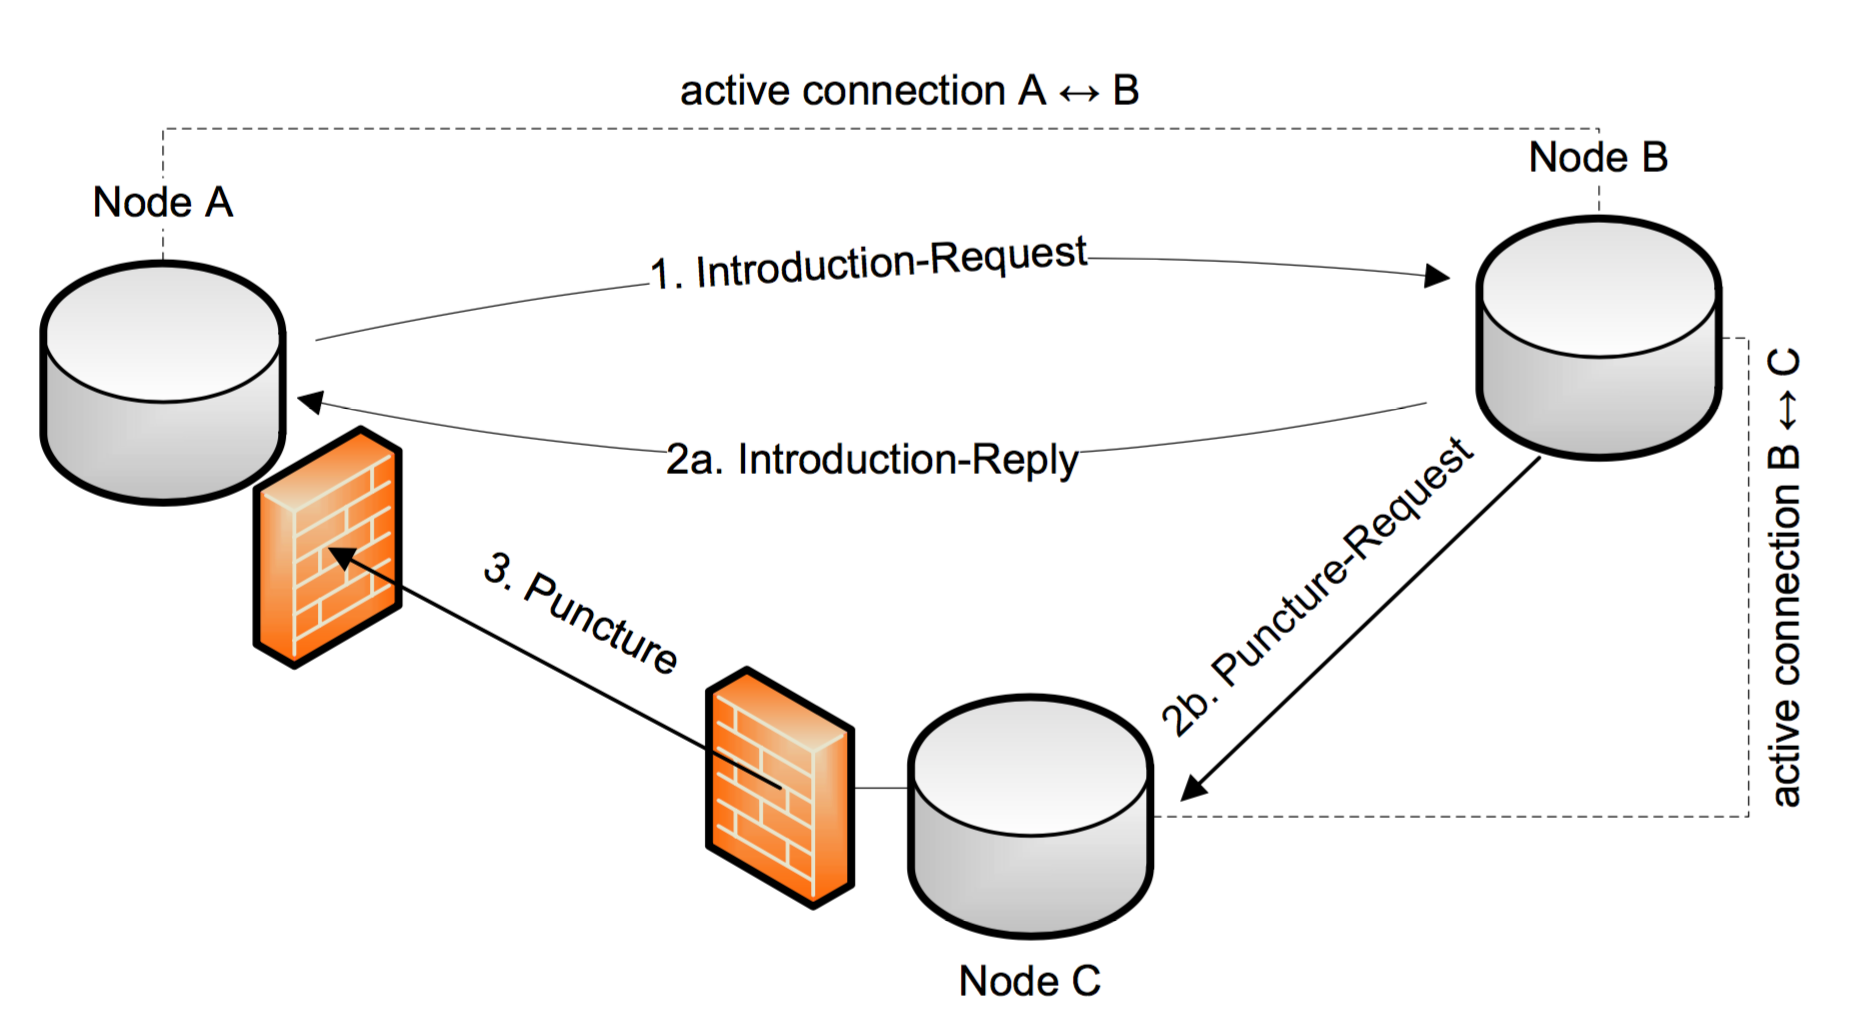
\includegraphics[width=0.7\columnwidth]{images/architecture/dispersy_discover}
	\caption{The discovery and NAT puncture mechanism as implemented in Dispersy.}
	\label{fig:dispersy-discover}
\end{figure}

The described mechanism will be replaced by a trusted walker that makes use of accumulated reputation in the Multichain, the accountant mechanism that keeps track of shared and used bandwidth, providing more reputation when a user provides bandwidth to help other users. The key idea is that sybil nodes, forged identities in the network, are ignored and not considered as a trusted peer since their reputation is low.\\\\
New peers in that network that have not built any reputation yet, start out by creating some random interactions with other nodes, learning about the network and the reputation of other users. With an interval, every node runs an algorithm to calculate the reputation of known peers. The amount of uploaded data does not have to be the only factor of this reputation mechanism: the uptime of the user in question can also be considered, where a higher uptime might lead to a better reputation. This leads to a trust network where each node inside the network knows about other trusted peers.\\\\
Peer discovery in this network 

\subsection{Libtorrent and Content Discovery}
Above the walker primitives explained in the previous Section, we find two components that are already present in the current system. The popular \emph{libtorrent} library is used to facilitate downloads. Libtorrent is written in C++, however interfaces for other programming languages such as Python, Go and Java are available. Libtorrent uses an alert mechanism to notify the program that is using the library about events in the library, such as download state transitions, peer discovery or completion of a metainfo lookup in the Distributed Hash Table (DHT). The current way of using \emph{libtorrent} in Tribler requires minimal changes to adhere to the proposed design, except for some optional refactoring and clean-up of the current code.\\\\
Currently, the methods to fetch peers from the DHT in \emph{libtorrent} is private and not accessible from Python. The current solution for this is to make use of a third-party library, named \emph{pymdht}, an implementation of the Mainline DHT protocol written in Python. This dependency is undesirable since it introduces some extra complexity and load of the system. Effort should be made to make the DHT method public so Tribler can get rid of the \emph{pymdht} dependency.
The content discovery components allows users to discover and search for available torrents, channels and playlists in Tribler\todo{afmaken}.

\subsection{libtribler}
Libtribler provides the interface to developers to make use of the above described primitives and contains the implementation of the REST API that is used to control and fetch data from \emph{libtribler}. The remainder of this Subsection will discuss the components that can be found at this layer in more detail.

\subsubsection{\textbf{Family filter}}
The freedom to upload any content users want, comes with a price. The legal aspect of the available content inside the network can be legally disputable. Legal content that is often undesired for most users is also available in a high number, such as sexual content. A mechanism is currently implemented in the Tribler core to filter out such explicit content, called the family filter. This filter is enabled by default and uses a list of keywords that can be associated with pornographic content. Unfortunately, this ad-hoc approach is not very effective since there are various false positives and negatives. While it does the job, it also demonstrates that the keyword-based approach can be greatly improved. However, we would consider this as an enhancement rather than a defect that prevents a correct usage of Tribler.

\subsubsection{\textbf{Video Server}}
The video server streams the video data to a video player outside \emph{libtribler} after or during downloads. The current implementation of the video server runs on a separate thread and is implemented using the \emph{SimpleHTTPServer} library, a built-in module that can be used to easily implement a HTTP web server. The video server is based on HTTP range requests, allowing the web server to serve a part of a file when the user seeks in a video.\\\\
The inner working of the video player is illustrated in Figure \ref{fig:video-server}. When the user starts playing a video in an external video player, the player performs a HTTP range request to the video server in Tribler. This range request contains information about the requested range of the video file in the header. When the video server contains the request, it first checks whether the requested range has been downloaded already. If so, the video server immediately returns the requested data in the HTTP response. If the requested range is not available, the video server notifies libtorrent that the  bytes in the requested range should be prioritized, reducing the latency before the requested range is completely downloaded. When all pieces are available, libtorrent notifies the video server and the video server completes the request by sending the data to the server.\\

\begin{figure}[h!]
	\centering
	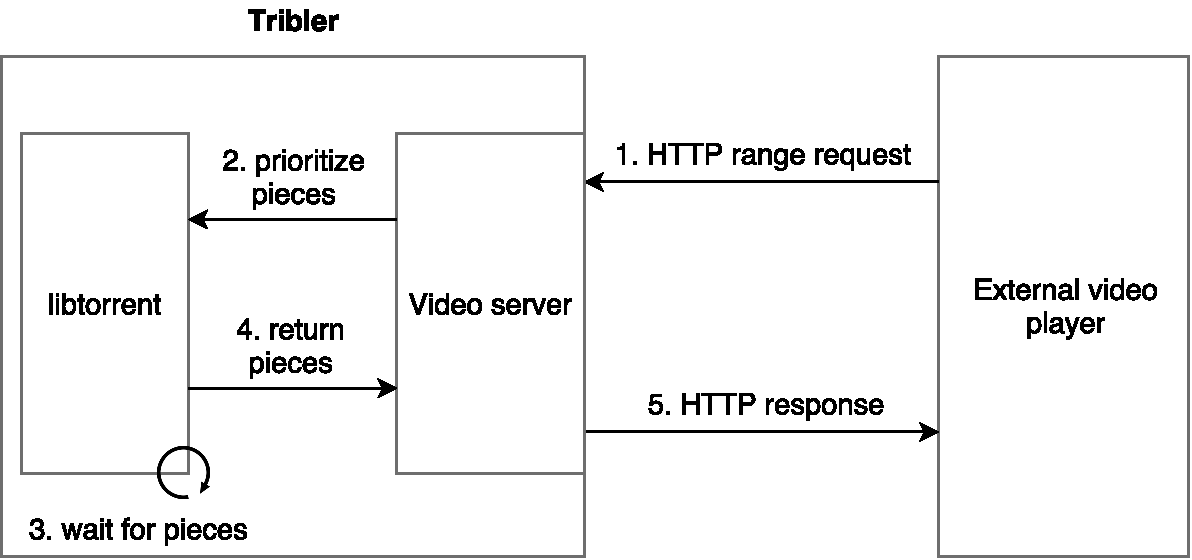
\includegraphics[width=0.7\columnwidth]{images/architecture/video_server}
	\caption{The inner working of the video server implemented in Tribler.}
	\label{fig:video-server}
\end{figure}

While the video server in the current form is functional, there is a major improvement that can be considered. The video player runs on a separate thread and uses blocking calls to wait for the buffer to be available. By integrating the video server inside the Twisted reactor thread, we can reduce complexity of this component and make use all of facilities that Twisted provides, for instance, for decoding a range request header. An additional consideration if performance is an issue, is to run the video server in a dedicated process. This might increase the complexity since a communication mechanism between the Tribler and video server process is required to inform libtorrent about the prioritization of pieces.

\subsubsection{\textbf{Credit Mining}}
The work on credit mining in a decentralized system has been extensively described by the work of Capot\k{a} et al\cite{capotka2015decentralized} and is defined as the activity performed by peers for the purpose of earning credit. These credits can be used for accessing new content or for receiving preferential treatment in case of network congestion. Although not shipped to users, A credit mining system (CMS) has been implemented in Tribler which is responsible for contributing bandwidth to the community, without any intervention of the user. This mechanism is displayed in Figure \ref{fig:credit-mining} and works as follows: first, the user selects a source of swarms for the system to take in consideration. Possible sources can be channels, RSS feeds or a directory of torrent files. Next, the CMS periodically selects a subset of the chosen swarms by the user. Finally, Tribler join the swarms and tries to maximize earned credits by downloading as little as possible and uploading as much as possible.\\

\begin{figure}[h!]
	\centering
	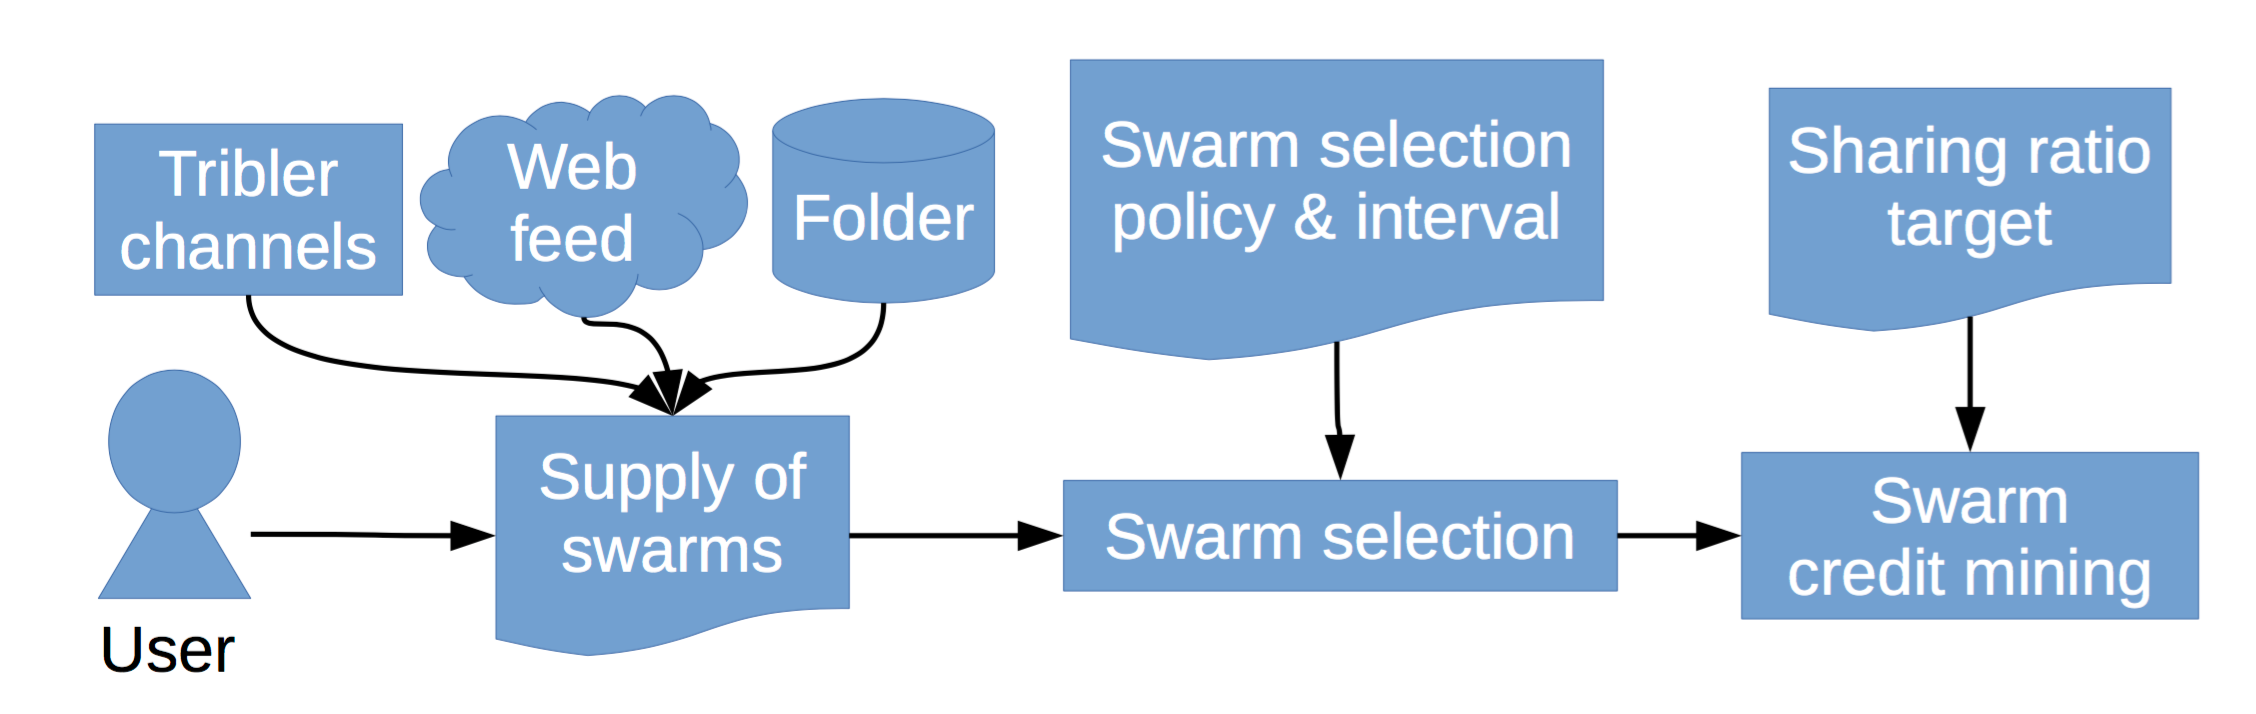
\includegraphics[width=0.7\columnwidth]{images/architecture/credit_mining}
	\caption{The credit mining system described in the work of Capot\k{a} et al.}
	\label{fig:credit-mining}
\end{figure}

CMS can apply different policies for swarm selection. A first policy is that it selects a swarm with the lowest ratio of seeders to all peers (where all peers consists of leechers and seeders). Intuitively, this boosts swarms that are under-supplied. The second policy is to select swarms based on their age. The intuition behind it is that newer content is often better seeded. The final policy that can be used is a random policy that selects a swarm with an uniform distribution.\\\\
This credit mechanism is a convenient way for users to build reputation by supplying bandwidth to the community. The Multichain can be used as accounting tool to keep track of upload and download rates.

\subsubsection{\textbf{Channel Management}}
Tribler allows users to create their own channel and share content within that channel. Content can be shared in the form of torrents and playlists where a playlist consists of a bundle of possibly related torrent, for instance, some episodes of a tv show. Users can add content to the channels of other users, providing that the owner of the channel has set the status of the channel to \emph{open}.

\subsection{Communication between GUI and \emph{libtribler}}
The communication between the upper level of the Tribler architecture, the GUI, and \emph{libtribler} is facilitated by a Representational State Transfer (REST) architecture. This architecture was introduced and defined by Roy Fielding in 2000\cite{fielding2000fielding} and is used frequently when building APIs that operate on the World Wide Web. A service that that conforms to the REST architecture, is called RESTful.\\\\
In a REST architecture, web resources are served to users, identified by Uniform Resource Identifiers (URIs). HTTP verbs (\emph{get}, \emph{post}, \emph{put} and \emph{delete}) are used to manipulate or retrieve these web resources. Operations can either be done on a collection of resources or on a specific resource\todo{table met verbs?}.\\\\
Prior to implementation of this API, we can already define some of the web resources. In Tribler, we can identify torrents, channels, playlists and downloads as resources that should be available for retrieval or modification using the API. Other than that, we might define a \emph{debug} object that contains various statistics that are tracked by Tribler so developers can build a debug panel which is helpful during development or performance measurements.\\\\
A REST API provides a very flexible and high-level interface that allows developers to write applications around Tribler, ranging from a command-line interface (CLI) to graphical appealing user interfaces. Moreover, the implementation of these utility applications are not bound to a specific programming language, providing a huge amount of implementation freedom. It also allows to run the user interface and Tribler in separate processes, improving responsiveness and testability.

\subsection{Graphical User Interface}
At the highest level of the Tribler stack, we find the user interface that is shipped to and used by end-users. The user interface should be able to communicate with the Tribler core using the REST API as described in the previous Subsection. Another critical component of the user interface is the ability to play and control a video. The current user interface uses the \emph{wxPython} bindings to the VLC player, however, this bindings are not functional on OS X due to platform incompatibilities.\\\\
The implementation of this interface is not limited to one programming language, however, to be able to reuse prior-existing code in the Tribler code base, it is a decent choice to write the interface in Python. Since the programming language is high-level and relatively easy to learn, new developers can easily make modifications to the user interface. We might also consider to refactor the current user interface to support the API. This consideration will be analysed in more detail in Chapter \ref{chapter:refactoring}. 

% http://delivery.acm.org/10.1145/2080000/2072433/p739-zeilemaker.pdf?ip=145.94.5.138&id=2072433&acc=ACTIVE%20SERVICE&key=0C390721DC3021FF%2E512956D6C5F075DE%2E4D4702B0C3E38B35%2E4D4702B0C3E38B35&CFID=816981133&CFTOKEN=23604061&__acm__=1469268778_0dc54a276c6ce7abce65547df9722e66
